\documentclass[11pt,final,fleqn]{article}\usepackage[]{graphicx}\usepackage[]{color}
%% maxwidth is the original width if it is less than linewidth
%% otherwise use linewidth (to make sure the graphics do not exceed the margin)
\makeatletter
\def\maxwidth{ %
  \ifdim\Gin@nat@width>\linewidth
    \linewidth
  \else
    \Gin@nat@width
  \fi
}
\makeatother

\definecolor{fgcolor}{rgb}{0.345, 0.345, 0.345}
\newcommand{\hlnum}[1]{\textcolor[rgb]{0.686,0.059,0.569}{#1}}%
\newcommand{\hlstr}[1]{\textcolor[rgb]{0.192,0.494,0.8}{#1}}%
\newcommand{\hlcom}[1]{\textcolor[rgb]{0.678,0.584,0.686}{\textit{#1}}}%
\newcommand{\hlopt}[1]{\textcolor[rgb]{0,0,0}{#1}}%
\newcommand{\hlstd}[1]{\textcolor[rgb]{0.345,0.345,0.345}{#1}}%
\newcommand{\hlkwa}[1]{\textcolor[rgb]{0.161,0.373,0.58}{\textbf{#1}}}%
\newcommand{\hlkwb}[1]{\textcolor[rgb]{0.69,0.353,0.396}{#1}}%
\newcommand{\hlkwc}[1]{\textcolor[rgb]{0.333,0.667,0.333}{#1}}%
\newcommand{\hlkwd}[1]{\textcolor[rgb]{0.737,0.353,0.396}{\textbf{#1}}}%
\let\hlipl\hlkwb

\usepackage{framed}
\makeatletter
\newenvironment{kframe}{%
 \def\at@end@of@kframe{}%
 \ifinner\ifhmode%
  \def\at@end@of@kframe{\end{minipage}}%
  \begin{minipage}{\columnwidth}%
 \fi\fi%
 \def\FrameCommand##1{\hskip\@totalleftmargin \hskip-\fboxsep
 \colorbox{shadecolor}{##1}\hskip-\fboxsep
     % There is no \\@totalrightmargin, so:
     \hskip-\linewidth \hskip-\@totalleftmargin \hskip\columnwidth}%
 \MakeFramed {\advance\hsize-\width
   \@totalleftmargin\z@ \linewidth\hsize
   \@setminipage}}%
 {\par\unskip\endMakeFramed%
 \at@end@of@kframe}
\makeatother

\definecolor{shadecolor}{rgb}{.97, .97, .97}
\definecolor{messagecolor}{rgb}{0, 0, 0}
\definecolor{warningcolor}{rgb}{1, 0, 1}
\definecolor{errorcolor}{rgb}{1, 0, 0}
\newenvironment{knitrout}{}{} % an empty environment to be redefined in TeX

\usepackage{alltt}

% basic packages
\usepackage[T1]{fontenc}
\usepackage[margin=1in] { geometry }
\usepackage{amssymb,amsmath, bm}
\usepackage{verbatim}
\usepackage[latin1]{inputenc}
%\usepackage[OT1]{fontenc}
\usepackage{setspace}
\usepackage{natbib}
\usepackage{enumitem}
\usepackage[hyphens,spaces,obeyspaces]{url}
\usepackage[font={bf}]{caption}
%\usepackage{pgfplots}
%\usepackage[font={bf}]{caption}
\usepackage{latexsym}
%\usepackage{euscript}
\usepackage{graphicx}
\usepackage{marvosym}
%\usepackage[varg]{txfonts}  Older version of ``g'' in math.
\usepackage{pdflscape}
\usepackage{algorithm}

% bibliography packages
\usepackage{natbib}
\bibpunct{(}{)}{;}{a}{}{,}
\bibliographystyle{apa}
\renewcommand{\bibname}{References}

% hyperref options
\usepackage{color}
\usepackage{hyperref}
\usepackage{xcolor}
\hypersetup{
    colorlinks,
    linkcolor={blue!50!black},
    citecolor={blue!50!black},
    urlcolor={blue!80!black}
}
\newcommand*{\Appendixautorefname}{Appendix}
\renewcommand*{\sectionautorefname}{Section}
\renewcommand*{\subsectionautorefname}{Section}
\renewcommand*{\subsubsectionautorefname}{Section}
\newcommand{\subfigureautorefname}{\figureautorefname}
\newcommand{\aref}[1]{\hyperref[#1]{Appendix~\ref{#1}}}
\newcommand{\algorithmautorefname}{Algorithm}

% packages for tables
\usepackage{longtable}
\usepackage{booktabs, threeparttable}
\usepackage{threeparttablex}
\usepackage{tabularx}
% dcolumn package
\usepackage{dcolumn}
\newcolumntype{.}{D{.}{.}{-1}}
\newcolumntype{d}[1]{D{.}{.}{#1}}
\captionsetup{belowskip=10pt,aboveskip=-5pt}
\usepackage{multirow}
% rotating package
\usepackage[figuresright]{rotating}
\usepackage{pdflscape}
\usepackage{subcaption}
\usepackage{caption} 
\captionsetup[table]{skip=5pt}

% packages for figures
\usepackage{grffile}
\usepackage{afterpage}
\usepackage{float}
\usepackage[section]{placeins}
\usepackage[export]{adjustbox}

% theorem package
\usepackage{theorem}
\theoremstyle{plain}
\theoremheaderfont{\scshape}
\newtheorem{theorem}{Theorem}
\newtheorem{assumption}{Assumption}
\newtheorem{lemma}{Lemma}
\newtheorem{proposition}{Proposition}
\newtheorem{remark}{Remark}
\newcommand{\qed}{\hfill \ensuremath{\Box}}
\newcommand\indep{\protect\mathpalette{\protect\independenT}{\perp}}
\DeclareMathOperator{\sgn}{sgn}
\DeclareMathOperator{\tr}{tr}
\DeclareMathOperator{\argmin}{arg\min}
\DeclareMathOperator{\argmax}{arg\max}
\def\independenT#1#2{\mathrel{\rlap{$#1#2$}\mkern2mu{#1#2}}}
\providecommand{\norm}[1]{\lVert#1\rVert}
\renewcommand\r{\right}
\renewcommand\l{\left}
\newcommand\E{\mathbb{E}}
\newcommand\dist{\buildrel\rm d\over\sim}
\newcommand\iid{\stackrel{\rm i.i.d.}{\sim}}
\newcommand\ind{\stackrel{\rm indep.}{\sim}}
\newcommand\cov{{\rm Cov}}
\newcommand\var{{\rm Var}}
\newcommand\SD{{\rm SD}}
\newcommand\bone{\mathbf{1}}
\newcommand\bzero{\mathbf{0}}
\DeclareMathOperator{\logit}{logit}
\DeclareMathOperator{\Cat}{Cat}
\DeclareMathOperator{\Multinomial}{Multinomial}

% file paths and definitions
\makeatletter
\newcommand*\ExpandableInput[1]{\@@input#1 }
\makeatother

% spacing 
\usepackage[compact]{titlesec}
\setlength{\parindent}{0pt}
\setlength{\parskip}{6pt plus 2pt minus 1pt}
\setstretch{1}

% appendix settings
\usepackage[toc,page,header]{appendix}
\renewcommand{\appendixpagename}{\centering Appendices}
\usepackage{chngcntr}
\usepackage{etoolbox}
\usepackage{lipsum}

% new commands
\newcommand\CPP{{C\texttt{++}}}
\newcommand\R{{\textsf{R}}}
\newcommand*\sameaff[1][\value{footnote}]{\footnotemark[#1]}
\newcommand\floor[1]{\lfloor#1\rfloor}
\newcommand\ceil[1]{\lceil#1\rceil}
\newcommand{\code}[1]{\texttt{#1}}

% subsubsection

\titleclass{\subsubsubsection}{straight}[\subsection]

\newcounter{subsubsubsection}[subsubsection]
\renewcommand\thesubsubsubsection{\thesubsubsection.\arabic{subsubsubsection}}
\renewcommand\theparagraph{\thesubsubsubsection.\arabic{paragraph}} % optional; useful if paragraphs are to be numbered

\titleformat{\subsubsubsection}
  {\normalfont\normalsize\bfseries}{\thesubsubsubsection}{1em}{}
\titlespacing*{\subsubsubsection}
{0pt}{3.25ex plus 1ex minus .2ex}{1.5ex plus .2ex}

\makeatletter
\renewcommand\paragraph{\@startsection{paragraph}{5}{\z@}%
  {3.25ex \@plus1ex \@minus.2ex}%
  {-1em}%
  {\normalfont\normalsize\bfseries}}
\renewcommand\subparagraph{\@startsection{subparagraph}{6}{\parindent}%
  {3.25ex \@plus1ex \@minus .2ex}%
  {-1em}%
  {\normalfont\normalsize\bfseries}}
\def\toclevel@subsubsubsection{4}
\def\toclevel@paragraph{5}
\def\toclevel@paragraph{6}
\def\l@subsubsubsection{\@dottedtocline{4}{7em}{4em}}
\def\l@paragraph{\@dottedtocline{5}{10em}{5em}}
\def\l@subparagraph{\@dottedtocline{6}{14em}{6em}}
\makeatother

\setcounter{secnumdepth}{4}
\setcounter{tocdepth}{4}

% title
\title{A Description of the IVI-NSCLC Model v1.0} 
\author{Devin Incerti\footnote{\href{http://www.thevalueinitiative.org/}{Innovation and Value Initiative}} \and Jeroen P. Jansen\sameaff}
\date{\today}
\begin{document}
\maketitle

\begingroup
 \hypersetup{linkcolor=black} \tableofcontents
 \listoffigures
 \listoftables
\endgroup

\clearpage
\phantomsection
\section{Open Source Value Project}\label{sec:osvp}

The continuing increase in U.S. healthcare costs has stimulated the introduction of initiatives to promote the use of high-value care.  Cost-effectiveness analysis can inform efficient use of healthcare resources by formally computing costs and benefits to identify the most valuable treatment options for a given disease.  In many countries, a single health technology assessment agency assesses the value of healthcare technology by means of cost-effectiveness analysis and recommends a utilization strategy. In the US, however, utilization decisions are decentralized and made by a variety of payers and provider organizations. Value frameworks are gaining prominence to guide utilization of therapies, but vary in perspective, the evidence considered, and approaches, thereby resulting in confusion and debate among stakeholders.

A thorough evidence-based analysis of the value of medical technology is resource intensive and complex.  Typically, there is no empirical study with sufficient long-term follow-up that compares all treatments for a particular disease regarding relevant clinical outcomes and costs. Thus, cost-effectiveness analyses generally rely on mathematical models that integrate evidence on the course of disease, treatment effects, and the relationship between clinical outcomes and costs, from a variety of studies. The nature of these evaluations can lead to disputes in the scientific literature and community. Models are typically difficult to understand. Even modeling experts may not be able to fully understand a model-based cost-effectiveness analysis without public source code and detailed model documentation. This lack of transparency also poses problems for users whose perspective, local context, or patient population varies from that of the reported analysis. In the absence of public access to the actual model, updating the evaluation is cumbersome, if not impossible, for someone other than the original model developer. As a result, published cost-effectiveness findings risk immediate irrelevance to some stakeholders and growing irrelevance to all stakeholders as new clinical evidence emerges. Value assessment only has relevance for decision-making when it reflects the totality of the latest evidence, is transparent, deemed credible by different stakeholders, representative of the local context and patient population, and can be easily updated without duplication of effort. 

With the Open-Source Value Project (OSVP), the Innovation and Value Initiative (IVI) aims to maximize both the relevance and credibility of value assessment in the context of the U.S. decentralized decision-making environment by developing and providing access to flexible open source decision models for value assessment. Refer to the IVI website {\href{https://www.thevalueinitiative.org/open-source-value-project/}{here} for a more detailed description regarding the objectives of these interactive models. 

IVI conducted its most recent OSVP within oncology. When selecting the tumor type of interest, IVI considered criteria such as burden of disease, development of innovative treatment, alternative treatment strategies available, availability of clinical evidence, and engagement of patient organization(s) to actively contribute to the project. 

Lung cancer is the leading cause of cancer related death worldwide. (1) Non-small lung cancer (NSCLC) accounts for an estimated 85\% of lung cancer cases and comprises adenocarcinoma, squamous cell carcinoma, and large cell carcinoma. (2) The five-year survival of stage IV NSCLC is less than 2\%. (3) Given the rapid pace of development in NSCLC, the scope of the OSVP needed to be limited to a very specific sub-population in order to ensure a model could be developed in a reasonable time frame that allowed IVI to demonstrate the typical areas of uncertainty in value assessment in oncology. The selected target population of interest for the most recent OSVP is metastatic epidermal growth factor receptor positive (EGFR+) NSCLC. EGFR mutations are more commonly observed in tumors from female patients with adenocarcinomas without a history of smoking and with Asian ethnicity, but can occur in patients with prior smoking history and across all races and genders.(4) The evidence base for the treatments used for the EGFR+ population is more modest than the evidence base for treatments used for EGFR negative NSCLC, which makes development of a model reflective of the latest evidence base more manageable given the logistical constraints set for this project. Future activities may include expanding the model to other subpopulations of interest.

\section{Purpose}\label{sec:purpose}
\subsection{Value assessment}
The IVI-NSCLC (egfr+) model is designed to assess the value of multiple competing sequential treatment strategies for patients with metastatic EGFR+ NSCLC. Sequential treatment strategies of interest are outlined in \textbf{Figure 1}. The final treatment strategies--starting with 1st line treatment (1L), followed by 2nd line treatment (2L), and treatment beyond 2nd line (2L+)--that can be evaluated with version 1 of the model were informed by the available evidence base, guidelines, and clinician input. The model is primarily designed to evaluate sequences starting with 1L, but sequences starting with 2L were analyzed given a certain 1L treatment received.

\textbf{Figure 1. Potential sequential treatment strategies of interest to be compared with the model} 

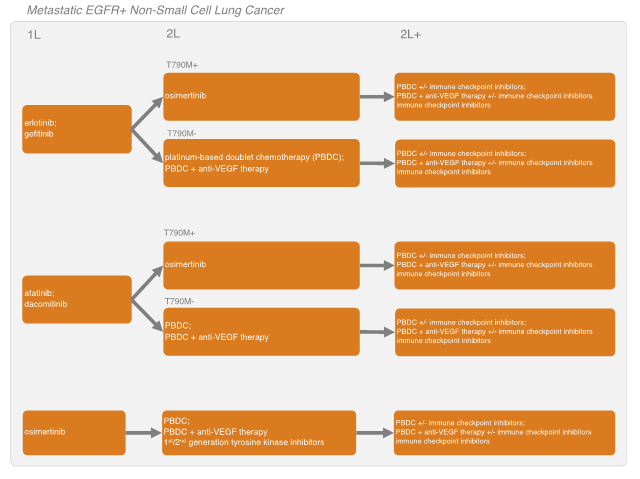
\includegraphics[scale=1]{Figure 1.PNG} 


The IVI-NSCLC(egfr+) model is suitable for informing decisions for specific (sub)populations, but is not suitable for making predictions at the individual level, nor should it replace the patient-physician shared decision-making process.  Local decision makers can modify the model to perform analysis of value that reflect the local setting while accounting for all scientific uncertainty and help them understand the confidence with which they make decisions. 
 
The IVI-NSCLC(egfr+) model is not a value assessment framework, but a model that simulates the costs, health outcomes, and risks associated with sequential treatment sequences for metastatic EGFR+ NSCLC. It can therefore be used with any value framework preferred by the user. Currently, two methodologies for decision analysis are supported by the model: CEA based on cost per quality adjusted life year (QALY) expressed as net-monetary benefit (NMB) and MCDA.(5) 

The MCDA was implemented according to Thokala et al. and based on the following criteria: progression free survival (PFS), overall survival (OS), adverse events, expected time on first, second, and third line treatment, utility/quality of life, health care sector costs, productivity losses, route of administration (oral/injection/infusion) and time the medication has been on the market.(6) The assessment of value can be performed from a health care sector perspective by only incorporating health care sector costs, or from a (limited) societal perspective by including productivity losses in addition.

Garrison, Kamal-Bahl, and Towse suggest five concepts of value that researchers should consider adding to the standard cost per QALY based CEA: (i) a reduction in uncertainty from a diagnostic test; (ii) insurance value for healthy individuals due to reduction against physical risk; (iii) the value of hope for individuals who become risk-loving and would rather pay for a therapy with a long right survival tail than a therapy with a shorter right survival tail but an equivalent (or shorter) expected life-expectancy; (iv) real option value when a therapy allows an individual to benefit from future medical innovations; and (v) scientific spillovers when the benefits of an innovation cannot be entirely appropriated by the innovator.(7)

The value of hope is most relevant for innovations that increase longevity and might be particularly well suited to the analyses of treatments for NSCLC.(7) This element of value revolves around the risk that a particular treatment may or may not work for a particular patient. Traditionally, CEA focuses on maximizing expected QALYs. However, patients might be willing to take gambles (i.e., they become "risk lovers") and care about the variation in benefits and costs, not simply the means. If patients value hope, they may prefer the treatment with greater variability in survival over the treatment with less variability despite having the same expected survival. In contrast, if patients are risk-averse, they may prefer the latter to avoid an unlucky outcome. Either way, they have a preference for one intervention over its alternative that appear identical based on its average costs and benefits. Patients may place substantial value on a modest chance of a durable survival response, over and above average survival, and decision-makers acting on their behalf may want to consider this aspect when making population level decisions regarding the value of interventions. 
Conventional value assessments focus on value to the sick, but recent research provides a framework for valuing medical technology for the healthy (i.e., "insurance value") as well.(8) The availability of an efficacious intervention for a certain disease state provides some degree of protection against the physical and financial risk among healthy individuals at risk for the disease. The insurance value framework can be implemented with knowledge of two additional parameters beyond those in conventional cost-effectiveness analysis: the probability of illness, and the marginal rate of substitution between the sick and the well states. 

The IVI-NSCLC(egfr+) model allows users to incorporate value of hope and insurance value into their analyses, while noting that these approaches are less well-established than conventional cost-effectiveness analysis. Future versions of the IVI-NSCLC(egfr+) may consider incorporating other value components, such as option value.


\subsection{Evaluation of scientific uncertainty}
Decision models can be used to inform efficient use of health care resources, but often lead to scientific disagreements and mistrust among stakeholders. Model inputs are typically informed by a formal evidence synthesis to ensure all relevant evidence is considered. However, decisions regarding the mathematical structure relating model inputs to outputs are frequently made arbitrarily based on the idiosyncratic expertise of the model developer without evaluating the impact on findings. While robustness can be assessed by means of sensitivity analyses, these are typically limited to studying the impacts of varying model inputs. For any given disease, a variety of modeling approaches have typically been proposed in the literature. In order to evaluate the impact of these different approaches on estimates of value in a systematic way, we need flexible open-source models to not only capture the uncertainty in model input parameters (i.e. parameter uncertainty), but also capture alternative model structures (i.e. structural uncertainty). This flexibility facilitates demonstrating the implications of different areas of uncertainty and leads to a better understanding of the reasons why value estimates can vary.

\section{Components}\label{sec:components}

Version 1 of the IVI-NSCLC(egfr+) model is designed to provide a starting point for open debate. To facilitate transparency, understanding, debate and collaboration among diverse stakeholders, the IVI-lung model will consist of the following components available in the public domain:

\textbf{Source code:} R and C++ code for the model are available in an IVI GitHub repository. Modelers and programmers may adapt the source code for their own purposes or collaborate to improve the code.

\textbf{R package:} The model will be released as an R-package with documentation available online. Researchers can use the package to run the model for custom analyses. Use of the package is recommended when performing analyses for scientific research.

\textbf{Detailed model documentation:} This document provides extensive technical details on the model structure, statistical methods for parameter estimation, and source data.

\textbf{Model Interface:} For users not well-versed in the programming language, a web application for running the model online is provided. The web application is designed for custom analyses and allows users full control over the treatments, patient population, model structures, parameter values, and simulation settings.

\textbf{Value Tool:} An important aim of OSVP is to obtain feedback from as many relevant stakeholders as possible. A general audience web-application has been developed, allowing those who are not experts in modeling or health economics, to interact with the model.

\section{Model structure}\label{sec:model-structure}

\subsection{Disease model}

The IVI-NSCLC is an individual-level continuous-time state transition model (CTSTM) in which patients can either have stable disease, progressed disease, or have died. To model sequential treatment strategies, we assumed that patients move to the next treatment after disease progression. In other words, a patient with stable disease moves to the second treatment in a sequence after progression on the first treatment, to the third treatment after progression on the second treatment, and so on. A patient can die at any time. \textbf{Figure 2} shows health state transitions for an example sequence of 3 treatments. Sequential treatment is incorporated into the CTSTM by expanding the number of health states according to the number of treatment lines. In the figure there are 3 treatment lines and 5 health states; more generally, there is one health state for each treatment line, a health state after progression on the final line, and a death state, so a model with n treatment lines will have n+2 health states. 

The hazard rate, $\ h^{qr} $ \textit{(u)} for a transition from state \textit{q} to state \textit{r} at time \textit{u} follows different parametric distributions including the exponential, Weibull, Gompertz, log-logistic, and fractional polynomial distributions as estimated with a multi-state network meta-analysis (NMA). In the individual-level model, time to each state \textit{r} that can be entered from state \textit{q} is sampled based on time-varying hazard rates and patients' transition to the state with the shortest sampled time.

The parameterization of transitions between health states allows incorporating potentially relevant prognostic factors or effect-modifiers. This would also facilitate including carry-over effects from one line of treatment to the next, once such data becomes available. 

\textbf{Figure 2. Simplified model structure with 4 states describing development of disease over time for a sequence starting with 1L, followed by 2L and 2L+ treatment; 2L+ treatment is captured with the L2 progression state}


\includegraphics[scale=0.3]{Figure 2.png} 


$\ S_{1} \textrm{ = Progression-free (stable disease) with 1L treatment }$

$\ P_{1} \textrm{ = Progression with 1L treatment }$

$\ S_{2} \textrm{ = Progression-free (stable disease) with 2L treatment }$

$\ P_{2} \textrm{ = Progression with 2L treatment, captures the survival with 2L+ without making a distinction between a progression free and progression phase }$

$\ D \textrm{ = Dead }$ 

$\ h^{S_{1}P_{1}} (u) \textrm{ = hazard for transitioning from progression-free to progression with 1L treatment at time \textit{u} } $ 

$\ h^{S_{1}D} (u) \textrm{ = hazard for transitioning from progression-free to dead with 1L treatment at time \textit{u} } $ 

$\ h^{S_{2}P_{2}} (u) \textrm{ = hazard for transitioning from progression-free to progression with 2L treatment at time \textit{u} } $ 

$\ h^{S_{2}D} (u) \textrm{ = hazard for transitioning from stable disease to dead with 2L treatment at time \textit{u} } $ 

$\ h^{P_{2}D} (u) \textrm{ = hazard for transitioning from progression on 2L to dead at time \textit{u} } $

\textbf{Figure 3. Simplified model structure with 3 states describing development of disease over time for a treatment sequence starting with 1L until death; 2L and 2L+ treatment is captured with the progression state} 


\includegraphics[scale=0.3]{Figure 3.png} 

$\ S_{1} \textrm{ = Progression-free (stable disease) with 1L treatment }$ 

$\ P_{1} \textrm{ = Progression with 1L treatment, captures the survival with 2L and 2L+ without making a distinction between progression free and progression phases }$ 

$\ D \textrm{ = Dead }$ 

$\ h^{S_{1}P_{1}} (u) \textrm{ = hazard for transitioning from progression-free to progression with 1L treatment at time \textit{u} } $

$\ h^{S_{1}D} (u) \textrm{ = hazard for transitioning from progression-free to dead with 1L treatment at time \textit{u} } $ 

$\ h^{P_{1}D} (u) \textrm{ = hazard for transitioning from progression on 1L to dead at time \textit{u} } $

\subsection{Adverse events}

The model includes multiple distinct adverse events associated with oncology treatment by treatment line. More precisely, for each treatment line and each patient, the model samples whether each adverse event occurs from a binomial distribution.

\subsection{Cost and utility}

All non-death health states are associated with utility and cost values. Cost values are separated into distinct categories (e.g., drug acquisition and administration costs, costs due to inpatient hospitalizations, etc.). Because we did not find strong evidence to the contrary, we assumed that utility and cost values remain constant over time within a given health state, but the model is also flexible enough to estimate utility and cost values that vary over time in a general manner. Adverse events cause utility decrements and more serious adverse events--such as those that require hospitalizations--increase health care costs. 

Drug acquisition and administration related costs are modeled based on standard clinical practice. For example, consider a case in which a therapy is dosed daily. Then costs will accrue each day until disease progression and the patient switches to the next treatment in the sequence. Another possible scenario is that dosing is based on fixed cycles. In these cases, costs will accrue until the end of a cycle or until the patient switches treatment due to disease progression. Other scenarios will be considered as required. 
Value of hope is illustrated with the model assuming representative relationships between utility values for each of the health states as a function of time reflecting risk-seeking and risk-averse behavior. 

Adverse events cause utility decrements and more serious adverse events--such as those that require hospitalizations--increase health care costs. 

\subsection{Patient heterogeneity}
The model is sufficiently flexible so that all model parameters (i.e., the parameters of probability distributions characterizing health state transitions, adverse event rates, costs, and utility) can depend on patient characteristics. In other words, we modeled input parameters as a function of covariates so that they can vary across individuals and treatments. That is, a given parameter, $\ a_{jt} $, for individual \textit{j} using treatment \textit{t} is modeled as $ \alpha_{jt} $ = $ \textit{g}^{-1} (X_{jt}\beta) $ where $ \textit{g}^{-1} $ (.) is an inverse transformation function. However, the extent heterogeneity can be modeled depends on the level of detail in the available evidence. We modeled heterogeneity based off of the level of evidence available. 

\subsection{Rationale for individual-level simulation}

Our primary motivation for using an individual-level model relates to the distinction between "clock forward" and "clock reset" approaches to parameter estimation. In the "clock reset" approach, time \textit{u} in $\ h^{qr} $ \textit{(u)} resets to 0 after each transition whereas in the "clock forward" approach, time \textit{u} refers to time since the start of the model. If a "clock reset" approach is used, then health state probabilities are calculated analytically using the Aalen-Johansen estimator and a cohort CTSTM can be used; conversely, if a "clock reset" approach is taken, then individual-level simulation-based approaches must be used to estimate health state probabilities. (9-12) In our case, the multi-state NMA is a mixture between the two: each time a patient begins a new treatment, time resets since separate multi-state NMA's will be conducted by treatment line, but time does not reset within a given treatment line since hazard rates depend on time, since treatment initiation is conditional on treatment line in the multi-state NMA. To accommodate a mixture of "clock reset" and "clock forward" approaches, we use an individual-level model. 

\section{Model outcomes}\label{sec:model-outcomes}

The model simulates the health outcomes, risks, and costs associated with alternative treatment strategies in oncology. The model's time horizon can be selected by the user and will default to a lifetime horizon. The health outcomes, risks, and costs will be combined to assess value using two frameworks: CEA and MCDA. Both disaggregated model outcomes and value estimates will be based on mean values (i.e., averages across all simulated patients). An overview of all model outcomes is shown in \textbf{Table 1.} Additional details are provided in the text below.  

\textbf{Table 1. Model outcomes} 

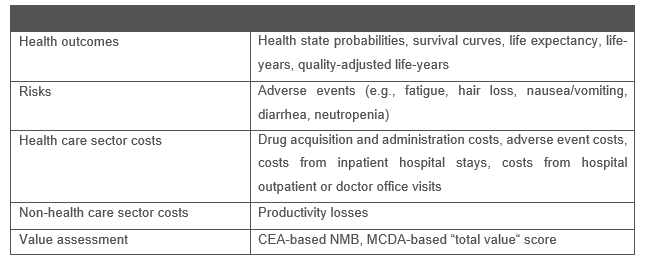
\includegraphics[scale=1]{Table 1.PNG} 

\subsection{Health outcomes}

The primary health outcome is the probability that a patient is in a given health state at a given point in time following treatment initiation. A survival curve was generated from the health state probabilities as one minus the probability that a patient has died. Since the model is an individual patient simulation, life expectancy is just the average time of death across simulated patients. Life-years was calculated as age at death minus age at treatment initiation. QALYs are weighted life-years, with weights equal to the utility values assigned to states.  Discounted QALYs were also calculated using a default discount rate of 3 percent.

\subsection{Risks}

The model calculates the expected number of adverse events per patient as the mean number of adverse events experienced by patients during the simulation. To improve interpretability, this number is reported as the expected number of adverse events per 1,000 patients. Both the expected number of total adverse events and the expected number of adverse events by type are reported.

\subsection{Costs} 

Costs are calculated for multiple categories and separated into health care sector and non-heath care sector costs as recommended by the Second Panel on Cost-Effectiveness in Health and Medicine.(13) Health care sector cost categories included drug acquisition and administration costs, adverse events costs, the costs of inpatient hospital stays, and costs from hospital outpatient and doctor office visits. Non-health care sector costs include productivity losses. We used both human-capital approach and friction-cost approach to estimate productivity losses associated with the different treatment sequences. The level of detail regarding productivity related cost estimates that were incorporated is based on the available data in the literature.

\subsection{Value assessment} 

Value was assessed using two frameworks: CEA and MCDA. If CEA is used for value assessment, then the value of treatment is estimated using the NMB. CEA from a societal perspective includes productivity losses while analyses from a health care sector perspective do not.

Value was assessed using two frameworks: CEA and MCDA. If CEA is used for value assessment, then the value of treatment is estimated using the NMB. CEA from a societal perspective includes productivity losses while analyses from a health care sector perspective will not. 

With MCDA, the value of each treatment strategy is based on a "total value" score. The score is calculated in three steps. First, a number of distinct criteria are assigned values on a common scale, for instance, ranging from 0 to 100. Second, each criterion is assigned points, say, ranging from 0 to 10, which is, in turn, used to calculate a weight by dividing each criterion's points by the sum of points across all criteria. For example, if there were 3 criteria and each criterion was given a score of 5, then each criterion would receive a weight of $ \dfrac{1}{3} $. If, on the other hand, the three criteria were given scores of 2.5, 5, and 7.5, then they would be given weights of 0.167, 0.33, and 0.5, respectively. Third, to aggregate results, we multiplied the value of each criterion on the common scale by its weight and sum the weighted scores across criteria. Future iterations of the model will consider using the Patient Experience Study to inform the baseline weights across attributes. 

\section{Source data and parameter estimation}\label{sec:source-data}

Key parameters for the model relate to: (i) the treatment effects of the interventions used for the different lines of treatment in terms of PFS and OS; (ii) utilities; (iii) healthcare resource use; and (iv) productivity.  Estimates for these parameters were based on currently available published evidence identified by means of a systematic literature review (SLR) and synthesized with meta-analysis techniques where appropriate.

\section{Simulation and uncertainty analysis}\label{sec:uncertainty-analysis}

\subsection{Parameter uncertainty}

Parameter uncertainty is quantified using probabilistic sensitivity analysis (PSA), which propagates uncertainty in the model input parameters throughout the model by randomly sampling the input parameters from their joint probability distribution.(14,15) Probability distributions are determined according to the distributional properties of the statistical estimates, which, in turn, depend on the statistical techniques used, and the distributions of the underlying data. \textbf{Table 2} displays the probability distribution that we used for the model parameters. When conducting a CEA, the results of the PSA are summarized using standard measures from the literature including cost-effectiveness planes, cost-effectiveness acceptability curves, and estimates of the expected value of perfect information.(16-19) Furthermore, all point estimates from a CEA or MCDA will be reported along with 95 percent confidence intervals. 

\textbf{Table 2. Probability distributions for probabilistic sensitivity analysis } 

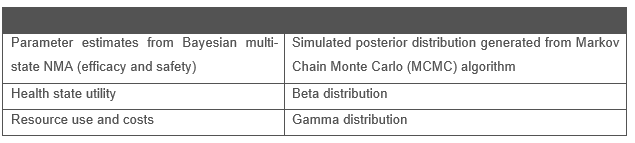
\includegraphics[scale=1]{Table 2.PNG} 

\subsection{Structural uncertainty}

Health state probabilities are typically very sensitive to the parametric distributions used in a multi-state statistical model. We explore this sensitivity by providing options to choose from a number of different distributions (e.g., exponential, Weibull, Gompertz, log-logistic, and fractional polynomial distributions). Furthermore, formal Bayesian model averaging was considered to generate point estimates derived from weighted averages of models fit using different distributions with weights based on posterior probabilities.(20)

In addition, as noted by the National Institute for Health Care Excellence (NICE) Decision Support Unit, methods for extrapolating outcomes beyond the time horizons of the original studies can have a large impact on results.(21) Moreover, the hazard rates and treatment effects on the hazard rate estimated using trial data may not generalize to the extrapolation period. As a result, we ran a number of scenario analyses to quantify the impact of different assumptions during the extrapolation period on results. These included: 

(a) Modeling health state transitions with different survival distributions (e.g., exponential, Weibull, Gompertz, log-logistic, and fractional polynomial distributions) during the extrapolation period;

(b) Modeling three separate treatment effect scenarios: (i) no difference in treatment effects across competing interventions, (ii) treatment effects are the same as during the pre-extrapolation period, and (iii) treatment effects diminish toward zero. 

Finally, different methods for simulating adverse events, costs, and utilities were considered as a review of the literature suggested that multiple approaches are scientifically valid.

\subsection{Implementation} 

The individual-level CTSTM was implemented using the R package \textit{hesim} developed by IVI. The package provides a general framework for integrating parameter estimates from a statistical model with different types of simulation models for economic evaluation. Parameter uncertainty is propagated throughout \textit{hesim} models using PSA. In our case, we randomly drew all input parameters from appropriate probability distributions, and simulated the CTSTM for each randomly sampled parameter set. All computationally intensive steps in \textit{hesim} simulation models are written in C++ so the simulations are fast enough to be run with a PSA in web applications. 


Although \textit{hesim} supports standard individual-level CTSTMs using R alone, the package also provides a comprehensive C++ library for developing custom simulations with C++. We took this approach by customizing \textit{hesim's} individual-level CTSTM classes and adding new features such as functions for simulating adverse events. 


 
\citet{baio2015probabilistic}

\begin{appendices}
\setcounter{table}{0}
\renewcommand{\thetable}{A\arabic{table}}
\setcounter{figure}{0}
\renewcommand{\thefigure}{A\arabic{figure}}
\setcounter{equation}{0}
\renewcommand{\theequation}{A\arabic{equation}}

\section{Systematic literature review}\label{app:slr}

\subsection{Treatment effects}

The systematic literature reviews of treatment effects focused on randomized controlled trials (RCTs) evaluating the efficacy of relevant competing interventions for the treatment of metastatic EGFR+ non-squamous NSCLC by line of treatment, i.e. 1L, 2L, and 2L+. Primary outcomes of interest were OS, PFS and time to progression (TTP). Details regarding eligibility criteria defining the scope of the studies considered relevant are outlined in Appendix Tables 1, 2 and 3. The identified evidence was used to estimate the relative treatment effects for each intervention versus a defined intervention of reference by line of treatment conditional upon the prior treatment (class), as well as to estimate the absolute treatment effects with the corresponding reference treatments.

\textbf{Appendix Table 1. PICOS criteria for review of treatment effects (metastatic 1L population)}

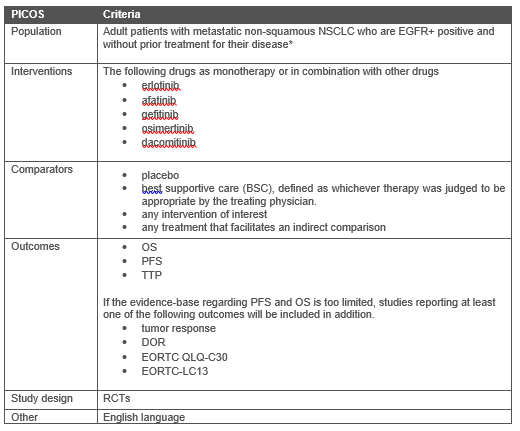
\includegraphics[scale=1]{Appendix Table 1.PNG} 

*Trials where the overall study population is an all-comer population, but subgroup results are reported for the target population of interest will be included; a trial or subgroup where the study population is a mixture of non-squamous and squamous  patients will be included of >90\% is non-squamous.

\textbf{Appendix Table 2. PICOS criteria for review of treatment effects (metastatic 2L population)}

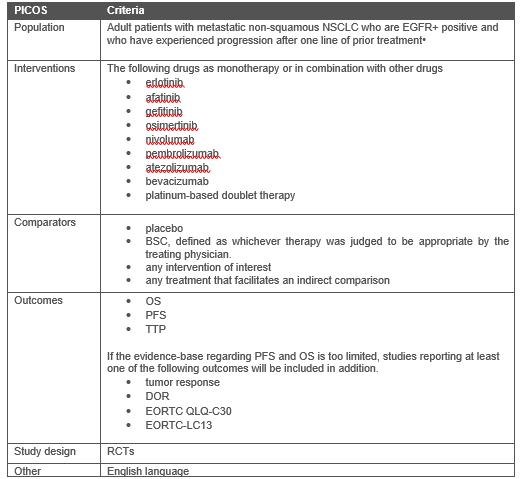
\includegraphics[scale=1]{Appendix Table 2.PNG} 

*Trials where the overall study population is an all-comer population, but subgroup results are reported for the target population of interest will be included; a trial or subgroup where the study population is a mixture of non-squamous and squamous patients will be included of >90\% is non-squamous.

\textbf{Appendix Table 3: PICOS criteria for review of treatment effects (metastatic 2L+ population)}

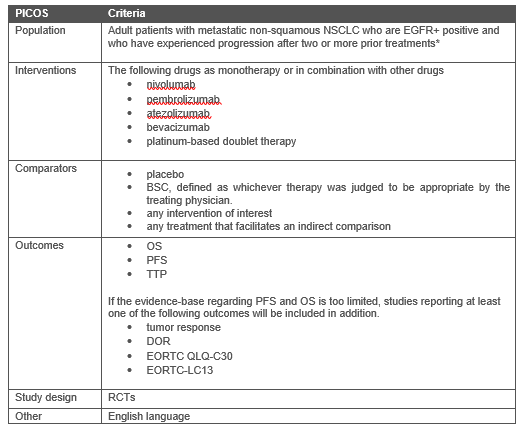
\includegraphics[scale=1]{Appendix Table 3.PNG}

*Trials where the overall study population is an all-comer population, but subgroup results are reported for the target population of interest will be included; a trial or subgroup where the study population is a mixture of non-squamous and squamous  patients will be included of >90\% is non-squamous. 

\subsection{Utilities}

Health state utility values (EQ-5d, HUI2, HUI-3, SF-6D) for the different health states were used in the model as well as disutility estimates associated with adverse events identified by focusing on review or overview studies. Furthermore, published mapping algorithms that allow a non-preference-based measure (generic or disease-specific measure) to be mapped onto a generic preference-based measure are of interest, as well as mapping algorithms between different generic preference-based health state utility values (e.g. between SF-6D and EQ5D) will be searched for. See Appendix Table 4 for study selection criteria.

\textbf{Appendix Table 4: PICOS criteria for review of utility estimates}

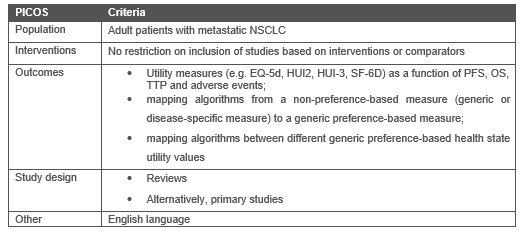
\includegraphics[scale=1]{Appendix Table 4.PNG} 

\subsection{Resource use, productivity, and cost}

Relevant evidence regarding resource use, productivity and cost estimates were identified by means of a review of published CEA modelling studies in NSCLC relevant for the US setting.  See Appendix Table 5 for study selection criteria.

\textbf{Appendix Table 5. PICOS criteria for studies providing information on resource use, productivity, and cost estimates} 

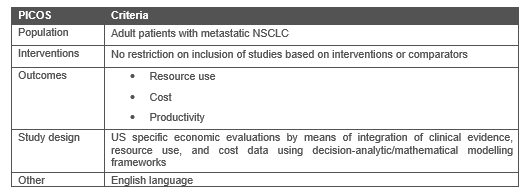
\includegraphics[scale=1]{Appendix Table 5.PNG} 

\subsection{Study identification}

Relevant studies were identified by searching the following databases using predefined search strategies: Medical Literature Analysis and Retrieval System Online (MEDLINE), Excerpta Medica database (EMBASE), and Cochrane Central Register of Controlled Trials. The study design filters recommended by the Scottish Intercollegiate Guidelines Network (SIGN) for MEDLINE and EMBASE were used to identify clinical trials. The search included terms related to the generic and brand name of the interventions of interest. The US National Institutes of Health Clinical Trial Registry and EU Clinical Trials Registry were also searched to identify completed clinical trials not yet published to identify any completed or ongoing trials that meet the criteria with results available.

For utility studies, and CEA studies providing evidence on healthcare utilization and costs, the following additional databases were searched in addition: NHS Economic Evaluation Database (NHS EED), Health Economic Evaluations Database (HEED), THe Health Economics Research Centre-maintained mapping algorithm database, and The University of Sheffield's ScHARRHUD database of health utilities' evidence.

Where there were gaps in the identified evidence, the search was expanded to include the grey literature, such as reports published by NICE.

\subsection{Study selection}

Two reviewers, working independently, reviewed all abstracts and proceedings identified in each of the searches according to the selection criteria, with the exception of outcome criteria in the efficacy and safety searches, which were only applied during the screening of full-text publications. All studies identified as eligible studies during abstract screening were then screened at a full-text stage by the same two reviewers. The full-text studies identified at this stage were included for data extraction. Following reconciliation between the two investigators, a third reviewer was included to reach consensus for any remaining discrepancies. The process of study identification and selection is summarized with Preferred Reporting Items for Systematic Reviews and Meta-Analyses (PRISMA) flow diagrams (including reasons for exclusion at both the abstract and full text screening stage). 

\subsection{Data collection}

For the clinical studies, two reviewers, working independently, extracted data on study characteristics, interventions, patient characteristics, and outcomes for the final list of included studies. Following reconciliation between the two reviewers, a third reviewer was included to reach consensus on any remaining discrepancies. For all outcomes of interest, information regarding point estimates, variability and uncertainty was obtained. For PFS and OS, hazard ratios and associated information regarding uncertainty were extracted. If results were reported as forest plots, the point estimate and 95\$ percent\ confidence interval were extracted using DigitizeIt software version 2.1.4 (Bormisoft - Informer Technologies, Inc.). Kaplan Meier curves will also be digitzed using DigitizeIt and the proportin of patients free of the event over time will be extracted and the number of patients at risk over time. Adverse events were collected, if reported. Data collected included number and percent of patients with: any grade 3 or 4 adverse event, any grade 3 or 4 treatment related adverse event, any serious adverse event, any treatment related serious adverse event, and death within 30 days of last treatment. The duration over which safety outcomes were reported were also captured. Discontinuation due to adverse events were also examined. 

For utility and cost-effectiveness studies, relevant information for the model was extracted from the source publications and checked by a second-reviewer. 

\subsection{Limitations}

Despite the strengths of the proposed SLR, some limitations are applicable to all SLRs that should be acknowledged. As the evidence base is continually growing, any trials published after the search date will not be captured. Further, any trials that are published close to the search date but are not yet indexed in the databases at the time of the search will not be captured by the search of MEDLINE, EMBASE, and Cochrane Central Register of Controlled Trials. As with any literature review, this SLR is limited by the use of published data. There is a risk of publication bias as some clinical studies fail to be published while others are published only in abstract form, which presents limited information. Finally, the search and selection were restricted to trials published in English.

\section{Network meta-analysis}

\subsection{Population, interventions, outcomes of interest}

Relative treatment effects between the competing interventions for the treatment of EGFR+ NSCLC were estimated by means of multiple NMAs, performed by line of treatment (i.e. 1L, 2L, and 2L+) conditional upon prior treatment (class) whenever feasible and relevant, based on data extracted from the studies identified with the SLR.(22,23) (For example, regarding 2L treatment, an NMA may be performed for a population that received a 1st generation TKI in the 1L, as well as an NMA for a population that received a 2nd generation TKI in the 1L setting.) The outcomes of interest were PFS, OS and adverse events. 

\subsection{Feasibility assessment}

With an NMA, interest centers on the comparison of the treatment effects of interventions that have not been studied in a head-to-head fashion. In order to ensure that these indirect comparisons of interventions are not affected by differences in study effects (i.e. known and unknown prognostic factors) between studies, we only considered the treatment effects of each trial. This consideration implied that all interventions indirectly compared have to be part of one network of trials where each trial has at least one intervention (active or placebo) in common with another trial. For interventions of interest that were not part of the same network, then it was not possible to perform an indirect comparison of treatment effects of these interventions without a substantial risk of bias.(22-24)

In combining direct and indirect evidence in an NMA, trials must be reasonably similar. Patients are randomized only within trials, not across trials, so there is a risk that patients participating in different trials differ with respect to demographic, disease or other characteristics. In addition, features of the trials themselves may differ. If these trial or patient characteristics are effect modifiers, i.e. they affect the treatment effects of an intervention versus a control, then there are systematic differences in treatment effects across trials. Systematic differences in known and unknown effect-modifiers among studies comparing the same interventions in direct fashion result in between-study heterogeneity. An imbalance in the distribution of effect modifiers between studies comparing different interventions will result in transitivity or consistency violations and therefore biased indirect comparisons.(25,26) 

In order to gauge the appropriateness of proceeding with an NMA, IVI's feasibility assessment included: (i) an assessment of whether the RCT evidence for the interventions of interest formed one evidence network for each outcome by line of treatment conditional upon prior treatment (class); and (ii) an assessment of the distribution of study and patient characteristics that may have had relative treatment effects across the direct comparisons of the evidence networks.

\subsection{Evaluation of consistency between direct and indirect comparisons}

Prior to the actual NMA, the consistency between direct and indirect comparisons were evaluated for networks that include closed loops. For comparisons (i.e., contrasts) that are part of a closed loop made up of more than 1 RCT connecting different interventions, we assessed the consistency by comparing the relative treatment effect for one contrast of this loop based on direct information with the corresponding estimates based on indirect information.(27)  

\subsection{Estimation of the relative treatment effects under the assumption of consistency}

Based on the findings of the feasibility assessment, the results of the RCTs that are part of one evidence network and deemed sufficiently similar were synthesized by means of NMAs by outcome of interest. Under the assumption of consistency, the NMA model relates the data from the individual studies to basic parameters reflecting the (pooled) relative treatment effect of each intervention compared to an overall treatment of reference. The NMA models were extended by incorporating covariates (i.e., meta-regression analysis) only if there was an imbalance in treatment potential effect modifiers across trials in the network.(28)

\subsection{Models, likelihood, priors}

We performed the NMA in a Bayesian framework.  Analysis within the Bayesian framework involves data, a likelihood distribution, a model with parameters, and prior distributions.  The model relates the data from the individual studies to basic parameters reflecting the (pooled) relative treatment effect of each intervention compared to an overall reference treatment.  For each outcome and line of treatment of interest, fixed and random-effects models were used.  Because some heterogeneity is always anticipated, we preferred a random-effects model.  When few RCTs are available, however, heterogeneity estimation can become unreliable, and the use of conventional 'non-informative priors' in the Bayesian framework can result in artificially wide uncertainty intervals.  Therefore, we stabilized the heterogeneity estimation by using moderately informative heterogeneity variance priors or used fixed effects models instead as needed.

\subsubsection{Progression-free survival and overall survival}

Traditional NMA for survival outcomes are based on hazard ratio (HR) estimates and rely on the proportional hazards assumption, which is implausible if the hazard functions of competing interventions cross.(29) Furthermore, separate meta-analyses of OS and of PFS data ignore the relationship between these outcomes. We performed NMA of OS and PFS that is based on a tri-state (stable, progression, and death) transition model where time-varying hazard rates and relative treatment effects are modeled with known parametric survival functions or fractional polynomials according to Equation 1 and illustrated in Appendix Figure 1.(29,30)

\textbf{Appendix Figure 1. Relationship between stable disease (S), progression (P) and death (D) as used in the multistate network meta-analysis model }


\includegraphics[scale=0.4]{Appendix Figure 1.png} 

$\ S_{ik} (u) \textrm{ = Progression-free (stable disease) in study i, treatment arm k at time u }$

$\ P_{ik} (u) \textrm{ = Progressed disease in study i, treatment arm k at time u }$

$\ D_{ik} (u) \textrm{ = Dead in study i, in treatment arm k at time u }$

$\ h_{ik}^{SP} (u) \textrm{ = Hazard rate for disease progression in study i, in treatment arm k at time u }$

$\ h_{ik}^{PD} (u) \textrm{ = Hazard rate for dying post-progression in study i, in treatment arm k at time u }$

$\ h_{ik}^{SD} (u) \textrm{ = Hazard rate for dying pre-progression in study i, in treatment arm k at time u}$

$\alpha_{.ik} $ represent the scale and shape parameters of the log hazard functions in study \textit{i} in treatment arm \textit{k}. $\mu_{.i} $ reflect the study effects regarding the scale and shape parameters in each study \textit{i}, $\delta_{0,ik} $ are the study specific true underlying relative treatment effects regarding the scale of the log hazard function for the transition from progression-free to progression, which are described by a normal distribution with an average effect for treatment t relative to reference treatment 1 (${d_{0,1t}}$) and between study heterogeneity $\sigma_{0}^{2} $. The treatment effects regarding the scale of the log hazard for the transition from progression-free to dead (${d_{3,1t}}$)and for the transition from progression to dead (${d_{6,1t}}$)as well as the treatment effects regarding the first shape parameters of the functions describing the transition rates (${d_{1,1t}}$, $d_{4,1t}$, $d_{7,1t}$)are assumed to be fixed by treatment.

The following competing survival distributions will be considered using this multi-state NMA framework: Weibull ($p_{1}=0$), Gompertz ($p_{1}=1$), and 2nd order fractional polynomials ($p_{1}={0,1}$ and $p_{1}={-1,0,1}$). These 2nd order fractional polynomial models are extensions of the Weibull and Gompertz model and allow arc- and bathtub shaped hazard functions. To facilitate parameter estimation, we assume treatment to only have an impact on the time-varying transition rates from stable to progression and stable to death; we assume transition rates between progressive disease and death independent of treatment. For the relative treatment effects in the 2nd order fractional polynomial framework we will assume that treatment only has an impact on two of the three parameters describing the hazard function over time (i.e. one scale and 1 shape parameter).

The model parameters will be estimated based on the number of patients in each of the three health states over time obtained from the published Kaplan-Meier (KM) curves for each arm of each trial included in the NMA. Accordingly, we will use a multinomial likelihood for the proportion of patients in each of the three health states at any point in time. These proportions are related to the time-varying hazards $\ h_{ik}^{SP} (u) $,$\ h_{ik}^{SD} (u) $, $\ h_{ik}^{PD} (u)$ according to a set of differential equations. (30) The prior distributions for the model parameters are:

\subsubsection*{Adverse events}

For adverse events reported as the number of patients experiencing the event, the NMA will be performed on the proportion of patients experiencing the event of interest with a binomial likelihood and logit link.(23)  For events reported as number of events per person-time by treatment (instead of number of persons with at least 1 event), we will use regression models with a log link function and Poisson likelihood. Normal non-informative prior distributions for the parameters were used with a mean of 0 and a variance of 10,000.

\subsection{Model selection}

The deviance information criterion (DIC) will be used to compare the goodness-of-fit of competing evidence synthesis models.(31) DIC provides a measure of model fit that penalizes model complexity. In general, a more complex model will result in a better fit to the data, demonstrating a smaller residual deviance. The model with the better trade-off between fit and parsimony has a lower DIC. A difference in DIC of about 10 points can be considered meaningful. Regarding PFS and OS, the DIC estimates will be used to select a subset of appropriate evidence synthesis models which are available for the end-user to choose from when running the simulations. Furthermore, the DIC estimates will be used for model averaging. Regarding adverse events, the DIC will be used to inform whether estimates obtained with a fixed or random effects approach will be used in the model simulations. 

\subsection{Software}

The parameters of the different models will be estimated using a Markov Chain Monte Carlo (MCMC) method implemented in the JAGS software package. JAGS will be run using R statistical software. (32)



\end{appendices}
\pdfbookmark[1]{References}{References}
\bibliography{references}


\end{document}